\documentclass[12pt, colorinlistoftodos]{article} 

\title{IAM: Impact Assessment \\ Elaboration d'un fichier de paramétrage fonctionnel}
\author{Merzereaud et al.}

\usepackage[frenchb]{babel}
\usepackage{ifthen} 
\newboolean{draft}\setboolean{draft}{false} % display notes, stamp

\providecommand{\main}{.}  % *Modification: define file location
% \usepackage{\main/.tex/setup}

\usepackage{tabularx}
\usepackage{eurosym}

% % Beginning of the setup file !!!!
% set up file for new commands and main packages :
% \providecommand{\main}{.}  % *Modification: define file location
\usepackage[utf8]{inputenc} % encoding
\usepackage[T1]{fontenc}
\usepackage{geometry}
\geometry{a4paper} % format de feuille
\geometry{top=2.5cm, bottom=2.5cm, left=2cm, right=2cm} %marges
%\linespread{1.5} % interligne

\usepackage[table,dvipsnames*,svgnames]{xcolor} % allow to put colour in table and correct a bug in names
% option 'gray' emulate a gray scale print of the document
\usepackage{fancyhdr}
\pagestyle{fancy}
\chead{\csname @title\endcsname}
\lhead{
\includegraphics[width=0.8cm]{\main/.tex/IAM_hex.jpg}}
\rhead{
\includegraphics[width=2cm]{\main/.tex/Logo_ifr_y.jpg}}
\lfoot{page \thepage}\cfoot{}
\rfoot{\csname @author\endcsname ~-~\the\year}

\fancypagestyle{plain}{%
    \fancyhf{}% clear all header and footer fields
    %\fancyfoot[L, R]{page \thepage}{\csname @author\endcsname ~-~\the\year} 
    \lfoot{page \thepage}\cfoot{}
    \rfoot{\csname @author\endcsname ~-~\the\year}
    \renewcommand{\headrulewidth}{0pt}%\
    %\renewcommand{\footrulewidth}{0pt}
}

\ifthenelse{\boolean{draft}}{
    %\usepackage{pagecolor} \pagecolor{darkgray} \color{lightgray}
    \usepackage[color={[rgb]{0.96, 0.77, 0.19}}]{draftwatermark}
    \SetWatermarkScale{4}
    \SetWatermarkText{DRAFT}
    \usepackage[backgroundcolor = orange]{todonotes}
}{ \usepackage[disable]{todonotes} }

\usepackage{marginnote}
\renewcommand{\marginpar}{\marginnote}

% using math
\usepackage{amstext}

\usepackage[hidelinks]{hyperref} % lien cliquables
\hypersetup{
colorlinks = true,
linkcolor = black,
citecolor = black,
urlcolor = blue
} % https://tex.stackexchange.com/questions/50747/options-for-appearance-of-links-in-hyperref
\usepackage{url}


\usepackage{array}
\usepackage{longtable}
\usepackage{float} 

\def\correction#1{%
    \abovedisplayshortskip=#1\baselineskip\relax\belowdisplayshortskip=#1\baselineskip\relax%
    \abovedisplayskip=#1\baselineskip\relax\belowdisplayskip=#1\baselineskip\relax}

\arrayrulewidth=1pt\relax
\tabcolsep=5pt\relax
\fboxsep=\tabcolsep\relax
\fboxrule=\arrayrulewidth\relax

\newcolumntype{A}[2]{%
    >{\minipage{\dimexpr#1\linewidth-2\tabcolsep-#2\arrayrulewidth\relax}\vspace\tabcolsep}%
    c<{\vspace\tabcolsep\endminipage}}

    %%%%%%%%%%%%%%%%%%%%%%%%%%%%%%%%%%%%%%%%%%%%%%%%%%%%%%%%%%%%%%%%%%%%%%%%%%%%%%%%%%%%%%%%%%%%%%%%%%%%%%%%%%%%%%%
    % Defining  table format
    \newenvironment{iTable}[3]{%
    \longtable{%
        |>{\centering$\displaystyle}A{#1}{1}<{$}% for inline equation
        |>{\centering}A{#2}{1.5}% for text
        |>{\centering}A{#3}{1.5}% for text
        |}\hline\ignorespaces}{%
    \endlongtable\ignorespacesafterend}

\newenvironment{cTable}[4]{%
    \longtable{%
        |>{\centering$\displaystyle}A{#1}{1}<{$}% for inline equation
        |>{\centering}A{#2}{1.5}% for text
        |>{\centering}A{#3}{1.5}% for text
        |>{\centering$\displaystyle}A{#4}{1}<{$}% for inline equation
        |}\hline\ignorespaces}{%
    \endlongtable\ignorespacesafterend}

\newenvironment{nTable}[6]{%
    \longtable{%
        |>{ \addtocounter{rowcntr}{-1} \refstepcounter{rowcntr} \therowcntr }A{#1}{1.5}<{\addtocounter{rowcntr}{1}} 
        |>{\centering$\displaystyle}A{#2}{1}<{$}% for inline equation
        |>{\centering}A{#3}{1.5}% for text
        |>{\centering}A{#4}{1.5}% for text
        |>{\small \centering}A{#5}{1.5}% for text
        |>{\centering$\displaystyle}A{#6}{1}<{$}% for inline equation
        |}\hline\ignorespaces}{%
    \endlongtable\ignorespacesafterend}

\newenvironment{not used}[1]{%
    \longtable{%
        |>{\centering$\displaystyle}A{#1}{1}<{$}% for inline equation
        |}\hline\ignorespaces}{%
    \endlongtable\ignorespacesafterend}
    %%%%%%%%%%%%%%%%%%%%%%%%%%%%%%%%%%%%%%%%%%%%%%%%%%%%%%%%%%%%%%%%%%%%%%%%%%%%%%%%%%%%%%%%%%%%%%%%%%%%%%%%%%%%%%%
\LTcapwidth=\textwidth % force width of longtable caption

\usepackage{ifthen}

\newcounter{rowcntr}[table]
\renewcommand{\therowcntr}{%
    \ifnum\value{rowcntr} > 0
    \ifnum\thetable = 30
        i\arabic{rowcntr}
    \else 
    \ifnum\thetable = 31
        p\arabic{rowcntr}
    \else
    \ifnum\thetable = 32
        t\arabic{rowcntr}
    \else
        \thetable. \arabic{rowcntr}
    \fi
    \fi
    \fi 
    \fi
}


\usepackage[export]{adjustbox}
\newenvironment{defbox}{% % a box with a title 'Glossary'
    \noindent
    \color{black}
    \adjustbox{innerenv={varwidth}{\dimexpr\linewidth-2\fboxsep-0.45cm\relax},
    margin=\fboxsep+.25cm \fboxsep+.2cm,frame,center}\bgroup  
}{%
    \egroup
}



\newcommand{\efmi}{%
    _{e,f,m,i}}
\newcommand{\efmc}{%
    _{e,f,m,c}}
\newcommand{\efm}{%
    _{e,f,m}}
\newcommand{\fm}{%
    _{f,m}}

\newcommand{\tabnl}{
    \tabularnewline\hline
}

\newcommand\Warning{%
 \makebox[1.4em][c]{%
 \makebox[0pt][c]{\raisebox{.1em}{\small!}}%
 \makebox[0pt][c]{\color{red}\Large$\bigtriangleup$}}}%

\newcommand{\pref}[1]{(\ref{#1})}

% % EOF setup.sty

\newcolumntype{L}{>{\(\displaystyle }l<{\)}} % math-mode version of "l" column type



\begin{document}

\thispagestyle{plain}

\begin{figure}
    
\includegraphics[width=\textwidth]{\main/.tex/header_ifre.png}
    \par ~ \par
    \begin{minipage}{\textwidth}
        \begin{center}
            {\huge \csname @title\endcsname }
        \end{center}
        \rule{7em}{.4pt}\par
        Mathieu Merzereaud$^1$, Claire Macher$^1$, Michel Bertignac$^2$, Marjolaine Fresard$^3$, Olivier Guyader$^1$, Christelle Le Grand$^1$, Sophie Gourguet$^1$, Florence 
        Briton$^1$, Maxime Jaunatre$^1$ \newline
        \par ~ \par
        $^1$ IFREMER ~| UMR AMURE, RBE/ Unité d'Economie Maritime \newline
        $^2$ IFREMER ~| RBE/ Unité Sciences et Technologies Halieutiques \newline
        $^3$ UBO ~| UMR AMURE
        \par ~ \par
        
        \begin{center}
            {\large \today }
        \end{center}
        
    \end{minipage}
\end{figure}
\hrule

\tableofcontents
\ifthenelse{\boolean{draft}}{
    \listoftodos
}{}
\newpage

\section*{Introduction}

IAM (Impact Assessment Model) est un modèle bio-économique de simulation de dynamiques de pêcheries, intégrant des outils spécifiques d'aide à la décision dans le cadre de mises en application théoriques de mesures de gestion. Ce document constitue un support d'utilisation du modèle, décrivant les étapes de paramétrage et de lancement des simulations, exposant les méthodologies et équations fonctionnelles utilisées en arrière-plan, et analysant les possibilités offertes par l'outil. Une première partie  principalement théorique décrira l'architecture modulaire du modèle, détaillera les paramètres mis en jeu ainsi que les liens fonctionnels les unissant. Les différents outils de simulation greffés au modèle "basique" et les méthodologies associées seront également présentés dans cette partie. Plus techniquement, la méthode de constitution du fichier de paramétrage fera l'objet d'une seconde partie, alors qu'une troisième et dernière partie décrira la mise en application des simulations au sein d'un environnement R.

\par~\par

Un effort particulier a été mis en œuvre afin que le modèle IAM possède un système de paramétrage  relativement simple à aborder, et ce malgré la diversité d'inputs qu'un modèle bio-économique multi-spécifique, multi-flottille et multi-métier induit. Pour cela, il a été convenu que l'intégralité des données d'entrée du modèle seraient contenue dans un fichier Excel d'extension ".xlsx", possédant une structure spécifique, et lisible par une procédure d'importation intégrée à l'outil (rappelons que le modèle IAM est utilisable dans un environnement R, et qu'un fichier de paramétrage type est disponible dans le package).
	
Le fichier d'entrée se compose des feuillets suivants : un feuillet "Stock" par espèce modélisée, un feuillet "Market", un feuillet "Flottille" par flottille modélisée, trois feuillets contenant les tables de conversions, un feuillet "Scénarii" et un feuillet "Stochasticité". Les seules données non intégrées dans le fichier et intervenant dans le modèle sont les options d'utilisation du modèle que l'on spécifiera séparément lors du lancement des simulations \todo{(cf partie 4)}.  	

\section{Feuillet "Stock"} \label{sec:stock}

Les feuillets de type "Stock" vont permettre de réunir tous les paramètres propres à chaque stock modélisé (paramètres biologiques, biomasses, effectifs totaux, mortalités par pêche,...). Il est possible de renseigner chaque paramètre de manière exhaustive au niveau historique puisque l'utilisateur peut décider du temps initial de la modélisation : ce fichier a donc aussi pour vocation d'être complété et remis à jour année après année afin que l'utilisateur aie à sa disposition une source de données à la fois évolutive et fonctionnelle.

\par~\par

Chacun de ces feuillets doit être nommé (click droit sur l'onglet $ \to $ Renommer) selon le schéma suivant : "Stock\_\_" +  nom de l'espèce sans espace (par exemple, "Stock\_\_Langoustine" ou "Stock\_\_Merlu\_commun".

\Warning La dénomination choisie sera également la caractérisation du stock dans le modèle (dans l'exemple, "Langoustine" ou "Merlu\_commun").

\par~\par

En haut de la feuille, un cadre jaune en partie protégé en écriture fait office de listing des variables considérées. La colonne "Variable" n'est pas modifiable : il s'agit des intitulés de chacun des paramètres tels qu'ils sont utilisés dans l'implémentation du modèle. L'autre champ fixe est le champ "Description" qui comme son nom l'indique présente rapidement les variables. La colonne "Alias" permet d'intégrer des tables de données dans lesquelles les variables ont un autre nom que le nom standard. Les deux colonnes "Variable" et "Alias" assurent ainsi la correspondance.  Enfin, le champ "Multi" est un multiplicateur utile dans le cas où les variables rentrées ne sont pas à l'unité standard décrite dans le champ "Description". Si une variable doit s'exprimer en tonnes, et que les valeurs inscrites sont en kilogrammes, il suffit d'insérer 0,001 dans la case correspondant à la variable en question, et la correction sera opérée lors de l'importation.

\par~\par

\Warning Il n'est pas obligatoire de renseigner toutes les variables déclarées ici (lire le champ Description pour plus de détails). Notons également que, par souci de facilité de traitement, la liste de variables intègre aussi les variables du feuillet "Market".

\par~\par

Il ne reste plus qu'à regrouper sur ce feuillet les tables susceptibles de décrire, pour l'espèce en question, les variables présentées dans le cadre jaune. Afin de faciliter ce processus, l'objectif fixé était de pouvoir gérer, lire et assurer le reformatage de tableaux de sources diverses, et de ce fait de multiples formats, tout en limitant au maximum les modifications à opérer sur les tableaux importés (ou copiés-collés) par l'utilisateur. Une macro développée spécifiquement pour ces fichiers permet de transformer les tables de paramètres insérées afin qu'elles soient lues par la procédure d'importation R. Prenons un exemple pour illustrer l'application ; soit un tableau historique d'effectifs totaux d'un stock quelconque inséré dans la feuille de calcul :

\begin{figure}[h!]
\begin{center}
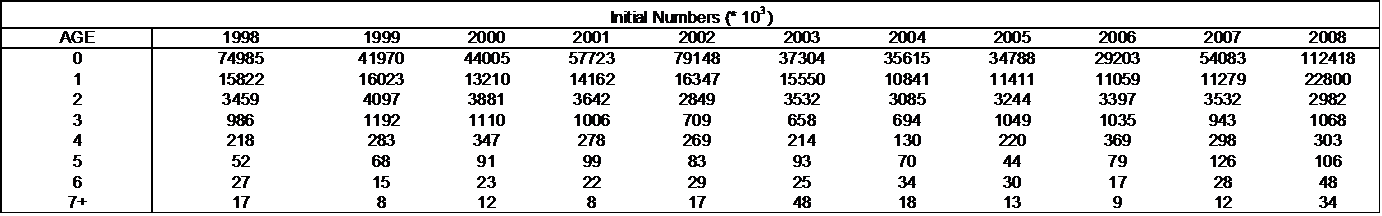
\includegraphics[width = \textwidth]{figures/param/stock1.png}
\end{center}
\label{fig:ex}
\end{figure}

Puisque les tables peuvent se succéder sur la feuille sans ordre prédéfini, il faut indiquer quelle variable est décrite par ce tableau. Il suffit pour cela de considérer cette appellation comme une variable, au même titre que la variable "âge" déjà déclinée, et insérer un nouveau champ comme ci-dessous (nous l'appelons "ini\_numbers") :

\begin{figure}[h!]
    \begin{center}
    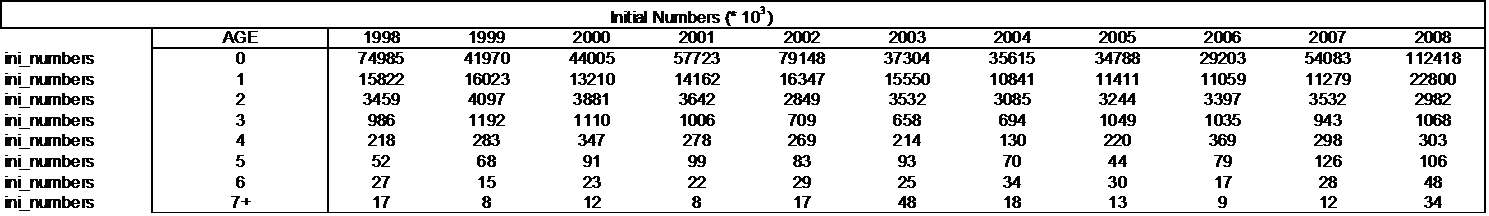
\includegraphics[width = \textwidth]{figures/param/stock2.png}
    \end{center}
    \label{fig:ini_num}
\end{figure}

Il faut maintenant le convertir en un tableau que la méthode d'importation saura lire. Appelons la macro "Préfixation" (Outils $ \to $ Macro $ \to $ Macros $ \to $ Préfixation $ \to $ Exécuter). Elle se présente sous la forme d'une petite interface :

\begin{figure}[H]
    \begin{center}
    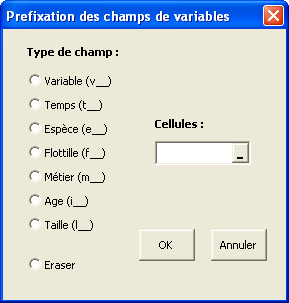
\includegraphics[width = 6.24cm]{figures/param/stock3.png}
    \end{center}
    \label{fig:prefix}
\end{figure}

Il faut alors caractériser les variables décrites dans le tableau au moyen d'un système de préfixation. Il s'agit de sélectionner les cellules à préfixer, puis de cocher la case correspondant au type de variable en jeu, et enfin de valider en cliquant sur OK. Pour recommencer, il suffit de cliquer sur le bouton dans le champ "Cellules :". La case "Eraser" permet de corriger les erreurs et d'effacer le(s) préfixe(s) de la plage sélectionnée. Cliquer sur "Annuler" lorsque le processus est terminé. On aboutit alors au tableau suivant :

\begin{figure}[h!]
    \begin{center}
    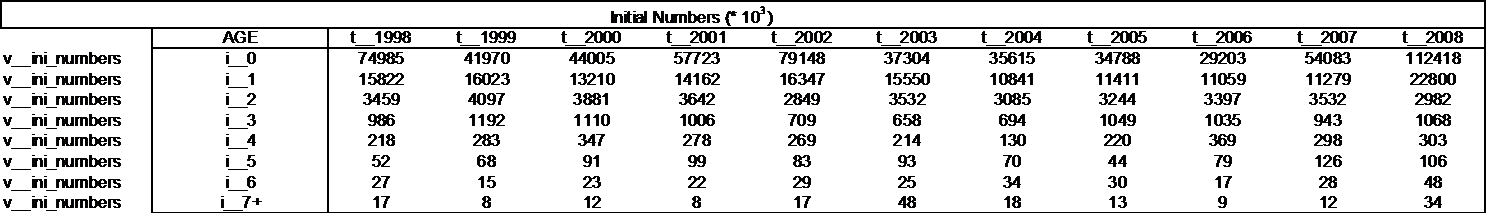
\includegraphics[width = \textwidth]{figures/param/stock4.png}
    \end{center}
    \label{fig:cancel}
\end{figure}
        
Le préfixe est composé d'une lettre spécifique à chaque type de variable, suivi de deux symboles "\_". Si besoin est, on peut rentrer l'appellation choisie pour la variable (ici "ini\_numbers") dans le champ "Alias" du cadre jaune, face à la variable correspondante (ici "Nit0"). Ce tableau est maintenant lisible par la méthode d'importation et sera affecté à la variable Nit0.

\par~\par

Il faut encore énoncer quelques règles au sujet du format et de l'organisation des tables de paramètres.  

\begin{itemize}
    \item[$\bullet$] Ne seront considérés que les champs de paramètres préfixés, ainsi que les numériques s'y rapportant. Dans la table précédente, les cellules "AGE" et "Initial Numbers ($*10^3$)" ne seront pas lues. 
    \item[$\bullet$] "\_\_" est un champ de caractères réservé aux variables : ne pas l'utiliser ailleurs dans le document (à part dans le nom des feuillets "Stock" et "Flottille", comme on va le voir).
    \item[$\bullet$] La dimension "Longueur" préfixée "l\_\_" ne peut définir des variables que si une clé tailles-âges est renseignée en tant que variable "alk".
    \item[$\bullet$] Les sauts de lignes (de taille quelconque) servent de séparateurs entre les tables à considérer.
    \item[$\bullet$] Une table peut se développer sur plusieurs successions de lignes ; par exemple, cette disposition est possible :
    
    \begin{minipage}{\linewidth}
        \centering
        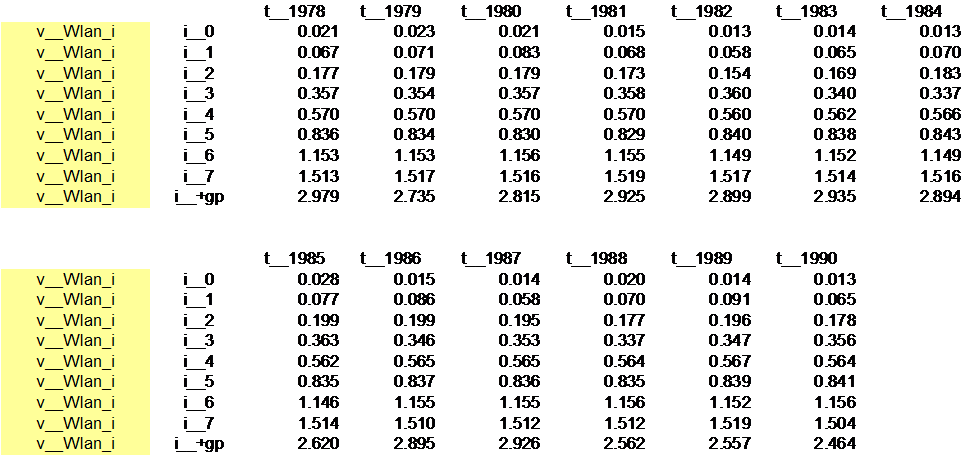
\includegraphics[width = \textwidth]{figures/param/stock5.png}
    \end{minipage}
    \vspace{12pt}

    \item[$\bullet$] au moins une variable doit être déclinée sur une colonne (comme "v" ou "i" dans la table précédente). La table suivante n'est, par exemple,  pas acceptée:
    
    \begin{minipage}{\linewidth}
        \centering
        
\includegraphics[width = 6.6cm]{figures/param/stock6.png}
    \end{minipage}
    \vspace{12pt}

    mais celle-ci l'est :

    \begin{minipage}{\linewidth}
        \centering
        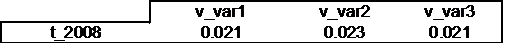
\includegraphics[width = 10.2cm]{figures/param/stock7.png}
    \end{minipage}
    \vspace{12pt}

\end{itemize}


Il est possible de définir les pas de temps à partir desquels définir la valeur initiale d'une variable pour laquelle un historique est disponible. La valeur initiale sera alors la moyenne sur les pas de temps choisis. Pour cela, il faut dédoubler le préfixe "t\_\_" sur les variables temporelles constituant le recul. Par exemple, si on veut une valeur initiale égale à la moyenne des 3 derniers instants (dans notre cas, les 3 dernières années) pour un temps initial égal à 2008, on a ce tableau :

\begin{figure}[h!]
    \begin{center}
    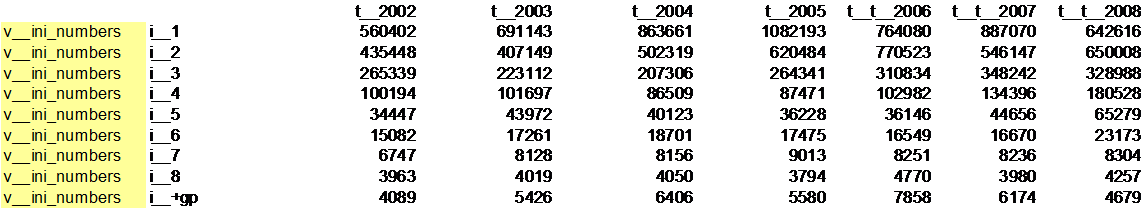
\includegraphics[width = \textwidth]{figures/param/stock8.png}
    \end{center}
    \label{fig:time}
\end{figure}

\Warning S'il a lieu d'être, le dédoublement du  préfixe temporel doit au moins être affecté à l'instant initial "t\_init", et potentiellement à des instants qui lui sont antérieurs. Pas de dédoublement signifie que le recul ne portera que sur l'instant initial. Notons que l'instant initial considéré sera déclaré lors de l'importation des paramètres. Toutes ces tables seront alors lues par la méthode d'importation et regroupées dans un objet R de type "liste".


\section{Feuillet "Market"}

Le feuillet "Market" diffère sensiblement des feuillets "Stock" par sa présentation générale, qui est similaire au format des feuillets "Flottille". Ceci s'explique par le fait que contrairement aux données de type "stock" qui proviennent le plus souvent de sources diverses (groupes d'évaluation,  expertises,...), les variables "Market" sont générées (au même titre que les variables économiques regroupées dans les feuillets "Flottille") par des routines d'extraction et de mise en forme standardisées. Il était donc plus facile de conserver ce format au sein du fichier de paramétrage. On se référera  donc au paragraphe décrivant le feuillet "Flottille" pour plus de précision. Notons simplement que ce feuillet comprend une colonne supplémentaire intitulée "categorie", pour des variables préfixées "c\_\_".

  
\section{Feuillet "Flottille"}

Ces feuillets vont regrouper les données économiques et d'activités des flottilles modélisées. Comme on vient de le préciser pour le feuillet "Market", toutes ces informations sont disponibles grâce à une routine développée en langage R, qui restitue  la donnée par flottille dans un unique format stable et reconnu par la méthode d'importation. Il suffira alors de compiler toutes les tables ainsi obtenues dans le fichier Excel,  en conservant la distinction "flottille" (1 feuillet par flottille) ou non, la seule restriction étant de conserver l'architecture standard des tables "flottille". Nous présentons maintenant ce format spécifique.

\par~\par

Ce tableau comporte 7 colonnes principales d'en-têtes \textit{nom\_variable}, \textit{libelle}, \textit{type d'indicateur}, \textit{flottille}, \textit{metier}, \textit{espece}, et \textit{indicateur}, dont voici la description :

\begin{itemize}
    \item[$\bullet$] \textbf{nom\_variable} : intitulé (préfixé) de la variable décrite tel qu'il sera utilisé dans l'implémentation du modèle (ôté du préfixe caractéristique des variables "v\_\_")
    \item[$\bullet$] \textbf{libelle} : descriptif de la variable
    \item[$\bullet$] \textbf{type d'indicateur} : catégorisation de l'indicateur
    \item[$\bullet$] \textbf{flottille} : champ facultatif. Variable flottille, préfixée "f\_\_".
    \item[$\bullet$] \textbf{metier} : champ facultatif. Variable métier, préfixée "m\_\_". Le niveau considéré est le niveau "métier éco", potentiellement différent du niveau considéré dans les feuillets "Stock".
    \item[$\bullet$] \textbf{espece} : champ facultatif. Variable espèce, préfixée "e\_\_".
    \item[$\bullet$] \textbf{indicateur} : champ facultatif. Valeur numérique de la variable.
    \item[$\bullet$] \textbf{…} : D'autres champs peuvent être ajoutés à droite de ces 7 premières colonnes, mais ils n'interviendront pas dans le processus de modélisation.
\end{itemize}

\par~\par

Les cellules non renseignées doivent rester vides. Toutes ces informations lues par la routine d'importation seront regroupées dans un nouvel élément "Fleet" de  la liste en sortie. Seules les variables déclinées par espèce seront intégrées à l 'élément "Stock" généré par les feuillets correspondants (cf section \ref{sec:stock}). Au même titre que les variables flottille, métier, temps,... les variables espèces doivent être consistantes dans l'intégralité du fichier. En conséquence, les dénominations des variables préfixées "e\_\_..." doivent être similaires à celle utilisées dans les noms des feuillets "Stocks" (par exemple, "Stock\_\_Sole\_commune" et "e\_\_Sole\_commune").

A titre indicatif, un document "FleetSpreadsheet" de tables types regroupant toutes les variables d'activité à renseigner est disponible au sein du package IAM. Il comprend une table complète assurant le paramétrage du modèle économique complet, ainsi qu'une deuxième table pour le modèle économique DCF.  


\section{Feuillet "fm\_matrix"}

Ce feuillet réunit les tables de distribution flottilles-métiers "bio" qui seront utilisées lors de l'étape de ventilation de la variable de mortalité par pêche. Ce processus pourra nécessiter en effet l'apport de la donnée de débarquements totaux par espèce au niveau flottille-métier "stock". Cette donnée n'étant disponible qu'au niveau flottille et flottille-métier "éco" dans les feuillets "Flottille" (variable $Lref$), une table d'allocation des débarquements par flottille pour chaque métier "stock" sera utilisée. Le feuillet contiendra une table par espèce modélisée (les métiers pouvant différer entre les espèces considérées), utilisant les notations habituelles décrites précédemment. Les valeurs peuvent être considérées comme les probabilités $P (metier | flottille \cdot espece)$.

\begin{figure}[h!]
    \begin{center}
    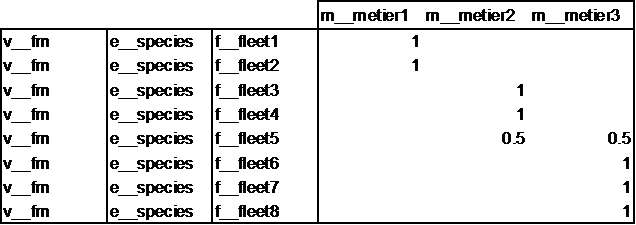
\includegraphics[width = 13.4cm]{figures/param/stock9.png}
    \end{center}
    \caption{Exemple illustratif d'une table "fm" pour une espèce donnée}
    \label{fig:fm}
\end{figure}


\section{Feuillet "mm\_matrix"}

Cette feuille intègre la matrice de transition entre le niveau métier "stock" utilisé par le modèle biologique, et le niveau métier "éco" qui caractérise ensuite le modèle économique. Elle sera utilisée au cours du processus engagé par le module "Market" (qui, on le rappelle, assure le lien entre les deux modèles, en redéfinissant notamment la dimension "métier"). La matrice contient ainsi des valeurs apparentées aux probabilités $P(espece \cdot flottille \cdot metier_{eco} | espece \cdot flottille \cdot metier_{stock})$.

\begin{figure}[h!]
    \begin{center}
    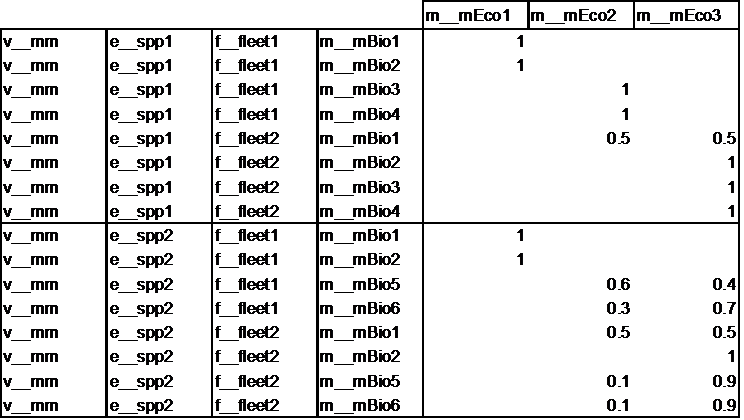
\includegraphics[width = \textwidth]{figures/param/stock10.png}
    \end{center}
    \caption{Exemple illustratif d'une table "mm"}
    \label{fig:mm}
\end{figure}


\section{Feuillet "icat\_matrix"}

Tout comme le feuillet "mm\_matrix", la donnée incluse dans cette feuille sera utilisée par le module "Market" pour procéder à un redimensionnement des variables. En l'occurrence, les tables "icat" vont participer à la conversion de certaines variables aux âges en variable par catégorie commerciale, permettant ainsi leur intégration ou leur application aux modèles de prix. Ces tableaux vont définir la distribution des catégories aux âges, et ceci par espèce. En d'autres termes, ils contiendront les probabilités $P(espece \cdot categorie commerciale| espece \cdot age)$.     

\begin{figure}[h!]
    \begin{center}
    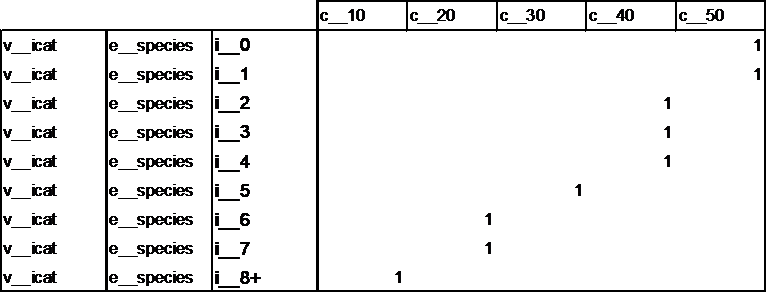
\includegraphics[width = \textwidth]{figures/param/stock11.png}
    \end{center}
    \caption{Exemple illustratif d'une table "icat"}
    \label{fig:icat}
\end{figure}


\section{Feuillet "Scénarii"}

Dans ce feuillet vont être consignées toutes les informations caractérisant les scénarios basés sur une intervention prédéfinie de l'utilisateur sur une ou plusieurs variables données \todo{(cf 1.2.6)}. Pour chacun des scénarios envisagés, une série de tables définissant les actions à opérer vont être insérées. Chacune d'entre elles décrit la variable à modifier, les dimensions sur lesquelles porte cette modification (pour quelle espèce, quelle flottille, quel métier, à quel instant,...?), et bien évidemment le multiplicateur à appliquer.

L'en-tête du feuillet est une partie bloquée en écriture qui présente les variables d'entrée et les variables internes qui pourront  faire l'objet d'un réajustement au cours de la simulation. Le nom de la variable composant chaque tableau devra donc se trouver dans cette liste. La première colonne de la feuille sert à caractériser le scénario : c'est ici que la première colonne de la table devra être inscrite, contenant le nom du scénario considéré. Une même table peut s'appliquer à plusieurs scénarios. Il suffit pour cela de séparer les noms de scénarios par "\&".Les colonnes suivantes constituent le tableau de valeurs, lequel suit les mêmes règles de constitution de tables que dans les feuillets "Stock" (cf section \ref{sec:stock}).

Notons pour finir qu'il est possible d'intervenir implicitement sur toutes les modalités d'une dimension donnée si on l'occulte dans la table correspondante. Par exemple, prenons une variable de dimension "flottille-métier-âge". Si la table ne se décline que suivant les dimensions "flottille" et "âge", les multiplicateurs s'appliqueront à tous les métiers pour la flottille et l'âge correspondant.

\begin{figure}[h!]
    \begin{center}
    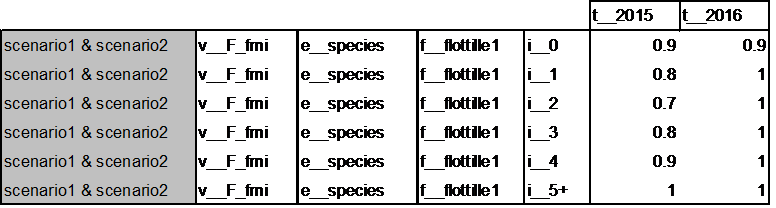
\includegraphics[width = 16.3cm]{figures/param/stock12.png}
    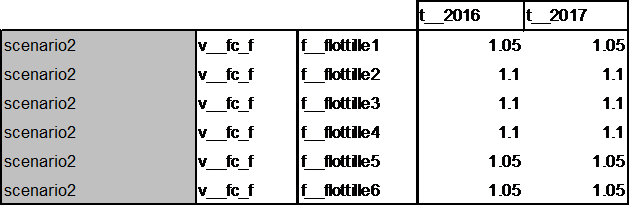
\includegraphics[width = 13.3cm]{figures/param/stock13.png}
    \end{center}
    \caption{Exemple illustratif d'un jeu de tables définissant 2 scénarios distincts}
    \label{fig:scenar}
\end{figure}


\section{Feuillet "Stochasticité"}

Cette feuille regroupe les paramètres régissant l'intégration de l'aspect stochastique dans le modèle, par l'intermédiaire de la donnée de recrutement (dans les futurs développements, la portée de la dimension aléatoire sera élargie à d'autres variables). Deux méthodes de simulation de recrutement sont paramétrables via cette feuille : un recrutement obtenu par tirage aléatoire dans un historique (la donnée doit être renseignée entre les deux balises "Samples" et "END Samples" dans une table préformatée, voir section\ref{sec:sample}), ou un recrutement comme étant la réalisation d'une variable aléatoire de loi paramétrable (la donnée doit être renseignée entre les deux balises "Random-variate" et "END Random-variate" dans une autre table préformatée, voir section \ref{sec:rand}).


\subsection{Table "Samples"} \label{sec:sample}

Ce tableau comporte 5 colonnes d'en-têtes \textit{Species}, \textit{TimeStep}, \textit{Value}, \textit{Mult}, et \textit{Weighted} :

\par~\par

\begin{itemize}
    \item[$\bullet$] \textbf{Species} : intitulé (préfixé) de l'espèce à laquelle se rapporte la donnée de recrutement.
    \item[$\bullet$] \textbf{TimeStep} : année du recrutement spécifié (non préfixé car n'intervient pas dans l'implémentation)
    \item[$\bullet$] \textbf{Value} : valeur de recrutement
    \item[$\bullet$] \textbf{Mult} : Multiplicateur de valeur. Si \textit{Value} est en milliers d'individus, \textit{Mult} devra être égal à 1000. La donnée finale doit toujours être en nombre d'individus.
    \item[$\bullet$] \textbf{Weighted} : Poids affecté à chaque année de recrutement dans le processus de tirage aléatoire. Permet de pondérer les chances d'être tiré au sort. Ces poids doivent être des entiers positifs (potentiellement nuls si on désire écarter certaines valeurs).
\end{itemize}

\par~\par

L'activation ou la désactivation de ces méthodes se décidera lors de la définition des "arguments" envoyés au modèle (cette étape sera décrite dans la quatrième partie de ce document). 
%L'
  
\begin{figure}[h!]
    \begin{center}
    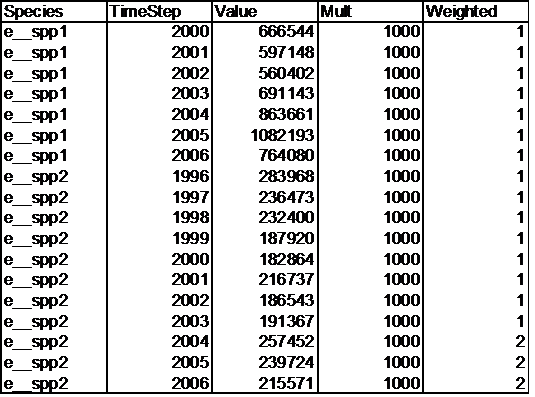
\includegraphics[width = 11.19cm]{figures/param/stock14.png}
    \end{center}
    \caption{Exemple d'une table "Samples". Ici, un historique sur deux espèces, avec tirage équiprobable sur la période 2000-2006 pour la première, et tirage sur 1996-2006 pondéré à l'avantage des 3 dernières années pour la seconde.}
    \label{fig:recru}
\end{figure}


\subsection{Table "Random-variate"} \label{sec:rand}

Cette table va caractériser les paramètres de la variable aléatoire dont la donnée de recrutement sera une réalisation. Elle comprend 5 champs qui sont la loi de distribution, les paramètres de cette loi (3 paramètres maximum à renseigner selon la loi), et l'espèce à laquelle s'applique cette loi de distribution de recrutement (ne pas oublier le préfixe "e\_\_" pour ce champ). L'en-tête du feuillet retrace les lois de probabilités potentiellement utilisables, ainsi que les noms des paramètres à renseigner pour chacune d'entre elles. De futurs développements permettront d'étendre cette application à d'autres variables que le simple recrutement.

\begin{figure}[H]
    \begin{center}
    
\includegraphics[width = 13.42cm]{figures/param/stock15.png}
    \end{center}
    \caption{Exemple d'une table "Random-variate". Ici, le recrutement de l'espèce considérée est une v.a de loi lognormale, et de paramètres $logmean=19,25...$ et $logsd=0,248...$ (cf en-tête du feuillet)}
    \label{fig:random}
\end{figure}


\end{document}